ss% \documentclass[sigplan,screen]{acmart}
\documentclass[sigplan,screen,review,anonymous,nonacm]{acmart}

% defining the \BibTeX command - from Oren Patashnik's original BibTeX documentation.
\def\BibTeX{{\rm B\kern-.05em{\sc i\kern-.025em b}\kern-.08emT\kern-.1667em\lower.7ex\hbox{E}\kern-.125emX}}

% Rights management information.
% This information is sent to you when you complete the rights form.
% These commands have SAMPLE values in them; it is your responsibility as an author to replace
% the commands and values with those provided to you when you complete the rights form.
%
\usepackage{graphicx}
\graphicspath{{figures/}}
% These commands are for a PROCEEDINGS abstract or paper.
\copyrightyear{2019}
\acmYear{2019}
\setcopyright{acmlicensed}
\acmConference[SOSP 2019]{SOSP 2019: ACM Symposium on Operating Systems Principles}{October 27--30, 2019}{Huntsville, Ontario, Canada}
\def\acmBooktitle#1{\gdef\@acmBooktitle{#1}}
\acmBooktitle{The 27th ACM Symposium on Operating Systems Principles October 27-30, 2019, Huntsville, Ontario, Canada}
% \acmPrice{15.00}
% \acmDOI{10.1145/1122445.1122456}
% \acmISBN{978-1-4503-9999-9/18/06}

\newcommand{\pjk}[1]{{\textcolor{blue}{PJK: #1}}}

\begin{document}

\title{Consensus Across Continents}

\author{Benjamin Bengfort}
\email{bengfort@cs.umd.edu}
\orcid{}

\author{Rebecca Bilbro}
\email{bilbro@gmail.com}
\orcid{}

\author{Pete Keleher}
\email{keleher@cs.umd.edu}
\orcid{}

\affiliation{%
    \institution{University of Maryland}
}

% Ben: when you read through the updated draft, can you make sure that we are making 
% Alia the star of the show rather than HC; e.g. talking about Alia as the framework 
% that implements HC, but in a uniquely flexible way?

\begin{abstract}
Distributing data storage systems across geographic areas provides resilience
to catastrophic failure and localizes user accesses, decreasing latency and improving 
throughput. 
However, as network distance increases, the impact of failure modes such as partitions 
and communication variability pose challenges to coordination that impair strong 
consistency.
As a result, geo-distributing systems implies a system size larger than a handful of 
replicas, requiring an extension of current consensus algorithms.
While some current systems are sufficiently large to protect against failures, they are 
also rigid, specialized for application-specific access patterns that do not generalize 
well. 
In order to balance consistency and performance in a multi-region context, geo -distributed
consensus must be flexible, adapting to changing network conditions and user behavior. 

In this paper we introduce Alia, a hierarchical consensus protocol that is designed for 
agility and serves as a framework to create large, strongly-consistent, and adaptable 
geo-replicated consensus groups. 
Alia splits coordination responsibility across two tiers: a root quorum responsible for 
moving the system through reconfiguration safely, and subquorums which manage direct
access to the data. 
Subquorums intersect with the root quorum using a novel method, delegated voting, which 
ensures that all replicas participate in both consensus tiers and provide transparent, 
linearizable guarantees across the entire system. 
This design ensures Alia can optimize throughput and availability by flexibly changing its 
configuration in real time to meet demand without sacrificing consistency. 
% Is the below sentence necessary?
%We demonstrate Alia's advantages and ability to scale to hundreds of replicas across more 
%than a dozen availability zones around the world using Amazon EC2. 
\end{abstract}

\begin{CCSXML}
<ccs2012>
    <concept>
        <concept_id>10002951.10003152.10003166.10003172</concept_id>
        <concept_desc>Information systems~Remote replication</concept_desc>
        <concept_significance>500</concept_significance>
    </concept>
    <concept>
        <concept_id>10002951.10003152.10003517.10003519</concept_id>
        <concept_desc>Information systems~Distributed storage</concept_desc>
        <concept_significance>500</concept_significance>
    </concept>
</ccs2012>
\end{CCSXML}

\ccsdesc[500]{Information systems~Remote replication}
\ccsdesc[500]{Information systems~Distributed storage}

\keywords{hierarchical consensus, geographic replication, delegated voting}

\maketitle

\section{Introduction}

% Don't really like this lead in or the megastore cite.
The availability of cloud services that span the globe has made it easier than ever
before to deploy geographically distributed data systems which replicate over 
continents and oceans. 
These types of systems increase local performance by minimizing network distance 
between users and replicas and provide the opportunity for data recovery in the face
of catastrophes such as floods or earthquakes. 
Moreover, the success of specialized, high-availability data systems~\cite{megastore} 
in maximizing throughput across the wide area has led to increased interest in 
geo-replication systems, particularly as more applications are being deployed with
international audiences in mind.
In order to generalize these systems, however, stronger consistency semantics are 
required to allow developers to reason correctly about the underlying behavior of 
the system. 

The most straightforward mechanism to guarantee strong consistency is to coordinate 
a group of replicas using distributed consensus, canonically represented by 
Paxos~\cite{paxos_simple} and its performance-optimizing 
variants~\cite{fast_paxos,multicoordinated_paxos,spaxos,generalized_paxos}. 
Although some recent research has explored the problem of geo-distributed consensus, 
specifically considering consensus with high latency links~\cite{mencius,epaxos}, 
the distributed consensus problem primarily considers the case of safety with either
one or two fail-stop node failures. 
Geo-replication, however, implies scaling; services running around the globe require
dozens if not hundreds of replicas, and introduces new failure modes such as network
partitions, where sections of the system operate independently without fail-stop 
failure, and highly variable latency that lead to changing network conditions. 
In order to scale systems beyond a handful of replicas, current 
systems~\cite{mdcc,calvinfs,spanner,scatter} use Paxos as a component, which can be 
instantiated across multiple transactions, shards, or tablets in order to manage 
subsystems that only require coordination between a few primary nodes. 

But Paxos alone is not enough; on the one hand we have consensus algorithms, which 
provide strong consistency for small quorums, but result in communication bottlenecks
at scale.
On the other hand we have real world systems, which can be engineered to scale 
consistency, but that rely on expensive hardware and complex, rigid designs,
and which cannot be made generally applicable. 

What is missing is the middle ground, a general framework for geo-distributed systems
that not only provides the highest possible throughput, but also the strongest 
consistency semantics in a network environment prone to correlated failures, 
partitions, and variable latency.
Such a framework should provide: 
\renewcommand{\baselinestretch}{1}
\begin{itemize}
    \item true horizontal scaling
    \item the ability to localize and optimize accesses to a variety of user patterns
    \item resilience beyond single node failure; e.g. in the face of partitions, but no 
    opportunity for partial or ambiguous failure
\end{itemize}
\renewcommand{\baselinestretch}{2}
% Ben: in the above, Pete asks 'why single node failure'?
It should moreover achieve these requirements with a single consensus layer, to facilitate 
implementation across a range of geographically distributed contexts, enable dynamic 
reconfiguration, and ensure straightforward system maintenance.

% NEEDS MORE!
This paper introduces the first such framework, \emph{hierarchical consensus}, a 
leader-oriented protocol that maintains multiple subquorums, each of which elects a leader 
to coordinate decisions. 
Hierarchical consensus coordinates all managed processes by organizing them into a tier
of quorums such that parent quorums manage the \emph{decision space} and leaf quorums
manage \emph{access ordering}.
Each tier implements quorums that make decisions about their respective operations.
To illustrate the fault tolerance, recovery properties, strong consistency guarantees, 
and throughput possible using the hierarchical consensus framework, we present Alia, the 
first distributed consensus protocol able to scale across hundreds of replicas around the 
world.

We begin by reviewing the problem of consistency across the wide area in Section 2. 
We present the high level details of the hierarchical consensus algorithm in Section 3, 
discussing the operations of the root quorum including delegated voting and epoch 
transitions.
In Section 4 we delve further into the operations of subquorums and transactions. 
In Sections 5 and 6, we demonstrate the safety and consistency guarantees of hierarchical 
consensus, and present the experimental results of the Alia system in Section 7.

\section{Background}
% assumptions we've made to get to this point
% why is geo-distribution hard and what solutions exist now?
% where we fit in the scheme of things - our design choices (e.g. we're a framework). 

We consider geographically replicated systems, which by their very nature scale to 
hundreds or thousands of processes working in concert to fulfill a myriad of client 
accesses from a wide area. 
The literature for such systems falls broadly into two categories; (1) new or optimized 
consensus algorithms designed to handle replication and failure in the wide area 
~\cite{epaxos, spaxos}, and (2) case studies of truly large-scale systems that implement 
distributed databases or other far-reaching applications~\cite{calvinfs,spanner,scatter}.
In this section, we will describe the algorithmic foundations for strong consistency 
and the systems that have been built upon them, both of which provide an intuition for
the design of Alia, a transparent, flexible framework that can offer strong 
consistency, horizontal scaling, and fault tolerance.

Modern cloud-scale applications developers are faced with geographic replication 
challenges routinely, but their options are limited to cloud service provider solutions 
~\cite{spanner} and theoretical works that do not consider scale 
~\cite{mdcc, epaxos, fast_paxos, vertical_paxos, wpaxos}.
Consider the trade-offs involved in designing a geographic replication system that must 
support a million users. 
One approach might privilege partition tolerance to ensure the operations can continue
even if large portions of the system are not able to communicate.
Another may allocate decision-making such that a few node failures will have no
impact on the overall state of the system.
Is it more important for decision-making to be efficient, requiring as few round-trips 
as possible, or for different parts of the system to be able to make decisions 
simultaneously?
There are many questions which must be addressed; what is the best mechanism for adding 
and removing nodes? 
Will many objects be accessed in different locations at different times?
How routinely will transactions require transatlantic commit?
These decisions require a balance between performance and throughput, between 
recovery and fault tolerance, and not to mention day-to-day systems administration.

\subsection{Geo-Distributed Consensus}
Geographic replication has two problems, the first of which is high and variable 
latency between links, which makes throughput slow between replicas across the wide 
area.
The second problem is a new type of failure, not of individual nodes, but partitions,
wherein two parts of a network are otherwise functional but unable to communicate.
Thus from the developer perspective, the goals are to minimize latency and to ensure
that quorums will not be disrupted by partitions.

To provide fault tolerance and strong consistency, we rely on quorum-based algorithms 
that coordinate different processes on different machines.
Largely these are all based on Paxos~\cite{generalized_paxos}, which has theoretically 
determined that the safest way to coordinate across nodes is a two-phase 
approach\textemdash a leader nominates itself, the rest of the nodes accept the leader, 
the leader proposes values, and that slot in the log is committed. 
This style of consensus creates a single log of operations that exists on all machines, 
and when it is applied in the same order, all replicas arrive at the same state.
From a performance perspective, the two-phase approach suffers from latency variability, 
and doesn't provide good throughput. 

As far as we are aware, only three Paxos variants\textemdash Raft, Mencius, and ePaxos
\textemdash have been used over the wide area. 
Raft attempts to eliminate the propose phase by pre-electing a leader responsible for the 
slots in the log.
Some other mechanism is then used to determine if the leader has failed, and to elect 
a new leader. 
Along with command aggregation, this optimization reduces the number of messages that 
have to be sent across the wide area.
This is good news for clients collocated with the leader, since they can expect the best
possible performance.
Raft is thus well-suited in a geo-replicated context for a primary backup replica 
scenario, particularly across local availability zones, and for catastrophic failure 
recovery.

However, Raft is not ideal for clients that are geographically distant from the leader.
An alternative option is Mencius, which assigns leadership in round robin fashion so that
there is a known, pre-elected leader for every slot.
This increases the likelihood that the client will be collocated with the leader for the 
best performance in the local area.
Thus, Raft and Mencius both improve performance for certain access problems, such as the 
case where clients are predominately located in a single portion of the consensus area, 
or are roughly evenly distributed across a small consensus area.

Like Mencius, ePaxos uses a multi-leader approach, but optimistically uses thriftiness 
and a fast path to make commits more quickly on behalf of the client.
This happens at the cost of a potential slow path during execution after the access is
completed, which requires even more coordination between replicas. 
These techniques give the best possible throughput when clients are uniformly 
distributed across all replicas, and can even avoid partial partitions by repairing 
logs with multi-hop consensus.
As conflict increases however, their advantages diminish. 

Though each of these three algorithms is useful in different contexts in the wide area, 
none scale. 
Consensus algorithms consider only single node failure and therefore only describe 
their behavior in the context of small quorums\textemdash three replicas allowing for 
one failure, or five replicas allowing for two to fail. 
As quorum size increases, the amount of coordination also increases, and so too does 
the amount of susceptibility to variable latency and partitions. 

% Unused content for Geo-Distributed Consensus subsection
% Consensus gives us consistency by maintaining a single ordering of operations that can be replayed all replicas can coordinate; this doesn't scale.
% Traditionally consensus considers small quorums (3 or 5) and think about small failures. 
% We don't consider quorum sizes of 7, 11,+ because performance deteriorates (Howard experiment). 
% Raft decreases in performance as size increases (should we use the figure from the first paper?) 
% These can only maintain consistency for the objects they manage. 
% No consideration for objects in adjacent consensus groups (this will lead to epoch discussion). 
% Raft does poorly across the wide area because it has a single leader that is in single region; everyone not in that region is forced to use high latency link to get to leader.
% Raft deals with partitions nicely because it selects a new leader in a new region. 
% Consider consensus in the WA where you have three replicas with different variable latencies the optimal scenario is to rely primarily on the replicas with the lowest latency. b/c of round robin leader assignment, Mencius improves the likelihood that accesses happen where the leader is (client collocated)
% ePaxos takes it a step further by always allowing the leader to be co-located with the client and hoping for the best
% ePaxos was designed for the wide area, because it can use thriftiness to adapt.
% However, ePaxos can't deal with conflict well and it also doesn't scale.
% these are components of other systems, not systems themselves. in the next section, see how they are used under the hood

\subsection{Engineering Solutions}
% In this section, let's try not to namedrop. Instead we should allude to components of well known systems that have tried to address the requirements in piecemeal fashion. 
%In real life, you need a namespace management layer, a lockserver, (etcd?) they hand out groups of related objects to replicas. then you need something to handle transactions, a system that coordinates multiple tablets and is single point of entry for client (this is 2pc). Then you need something to handle access to the tablets & replicate writes to disk (ceph)
% A "standard" solution that describes Calvin, Spanner, and MDCC well is as follows:
% - etcd for namespace locking and leases 
% - xyz (MySQL maybe? Calvin? JBoss? Narayana?) for transactions -- need to come back to this
% - Ceph or other distributed system for replicated accesses 
% - Time systems or vector clocks
% These systems aren't bad, but they were designed for a specific purpose in mind. Without focusing on consistency in the wide area. The result is that they are inflexible and brittle, but very good. not generally applicable. We are using the lessons learn from these systems to recognize that flexibility is ultimately the most important require to solve wide area consistency. Now that we've seen it, we can make better statements about what's required. 
% Why are we describing this? It shows how inflexible engineering systems are, and our response. It also shows the possibility of partial failure.
In the previous section, we considered consensus in the wide area for strong 
consistency. 
For geographically distributed systems in the wild, the chief practical consideration 
is high throughout. 
% say on the order of how many?
This is achieved by partitioning the namespace into tablets of related objects that are 
managed together, and by placing those tablets in geographic proximity to their users. 
% Ben: Pete expressed confusion about the below sentence; perhaps add citations?
Early systems sacrificed availability for the sake of consistency, but today's strongly 
consistent systems use a complex architecture that depends on high performance data 
center hardware to make specific guarantees.

\begin{figure}
\caption{Example of a general geo-distributed system architecture}
\centering
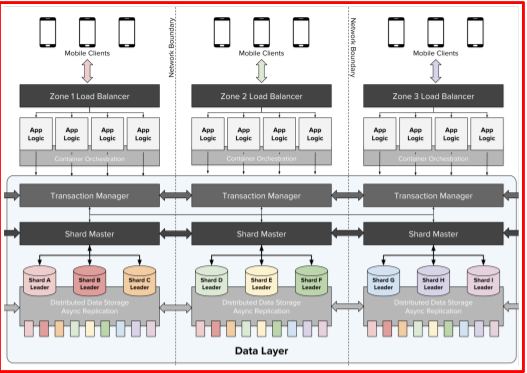
\includegraphics[width=8cm]{figure_1_general_architecture.png}
\label{fig:general_architecture}
\end{figure}

An architecture for a general geo-distributed system is shown in figure \ref{fig:general_architecture}.
A lockserver such as etcd~\cite{etcd_raft} or Chubby~\cite{chubby} assigns tablets to 
either individual replicas or to small quorums. 
Accesses go through these quorums and are written to a distributed data store or a file 
system such as Collossus~\cite{gfs} or Ceph~\cite{ceph}.  
The replicas or quorums routinely renew their leases with the lockserver, but if they die 
or the lease expires, the tablet can be reassigned to another replica that can read the 
data off the geo-distributed file system.
For cross-tablet accesses, the state of the art is to use snapshot isolation with 
extremely precise timestamps or vector clocks. 
The benefit of this architecture is that the primary workload is handled by small quorums 
of the type described in the previous section. 
Moreover, the system is extremely robust to node failures, meaning they provide insurance
against data loss.

Together, the three primary components of such systems\textemdash the name service, 
lock service, and distributed file system\textemdash achieve the foremost requirement: 
high performance for many simultaneous users.
However, these system components are not safer merely because they operate 
independently from the rest of the system; a data store is not less susceptible to 
latency or more resilient to failure by virtue of being engineered separately from 
the lock server or name server.
Their disjunction does not furnish any particular advantage; on the contrary, it
introduces several new challenges.

First, the consistency properties are handled at multiple layers, adding complexity
that makes it very difficult to reason about system-level consistency in a meaningful
way.
% Ben: Pete suggests adding an example to illustrate the above.
The lockserver can become a bottleneck; the primary replica, responsible for ordering
accesses, may become imbalanced; and finally, the distributed data layer may have a
completely difference consistency semantic.
This means that such systems must rely on regular human intervention and coordination 
for administration and maintenance.

Moreover, the separation of decision-making across the components of these systems makes
them extremely rigid; depending, for instance, on coarse epochs and expensive hardware 
to provide safety, and assuming, rather optimistically, that tablets will be accessed 
only inside a single region. 
% Ben: to the above sentence, Pete says "MCCS?"
Optimization for geographic accesses is thus necessarily very naive; executed via 
applications that store, as an example, the entirety of a user's inbox in a single 
location in spite of having more than enough data on usage patterns to inform a more 
nuanced, even adaptive, storage strategy.

While these systems work, they are fundamentally limited by their design.
What they really need is a mechanism for achieving the same high throughput 
and strong consistency without incurring the expenses of human coordination and the 
loss of system-wide interpretability.
Most importantly, they should also provide the flexibility of the algorithmic 
approaches, endowing engineered systems with the opportunity to adapt to changing 
conditions, and untethering them from reliance on premium hardware.
% Ben: to the above sentence, Pete says the algorithm v engr dichotomy is not sufficiently clear
An example of a system designed using a single consensus layer is shown in figure
\ref{fig:simplified_architecture}.

\begin{figure}
\caption{A simplified architecture with a single consensus layer}
\centering
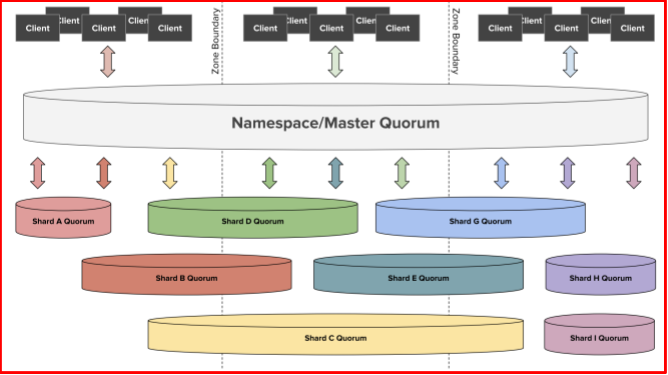
\includegraphics[width=8cm]{figure_2_simplified_architecture.png}
\label{fig:simplified_architecture}
\end{figure}

% Unused content for Engineered Solutions subsection
% geo-specific examples
% before two blocks were in the same AZ, but the 3rd was in another
% but now you have at least 2 blocks in one region and another roaming
% in the old system , you have to redo the system. 

\subsection{A Framework for Agile Systems}
% This will be a very short section with bullets with bold short description and longer plain description for each. Use the previous two sections to describe the design requirements that our system will end up fulfilling

% Is this too much like Eris?
Alia takes a different approach to implementing geo-distributed systems, focusing
on a system's ability to be \emph{flexible}. 
Flexibility ensures that the system can balance requirements for throughput and 
availability while still maintaining the strongest possible consistency semantics.
To achieve this, Alia is based on three primary design requirements that inform the 
rest of the framework.

\emph{Requirement 1: Systems should be as fluid as the information they contain.}
Many systems are optimistic, they assume that conflict is rare and that objects are 
accessed in standard patterns that change. 
In our experience, both people and information flows freely therefore a system must
accommodate organic and shifting usage patterns; for example a set of objects may 
primarily be accessed only in daylight, requiring the system to adapt by moving the
coordinating replicas to the locales currently in working hours. 
To accommodate this requirement, Alia is designed to regularly and safely transition 
through reconfigurations called epoch changes, reallocating replicas into subquorums 
to manage specific partitions of the namespace. 
Epoch changes are \emph{fuzzy} to ensure that reconfiguration does not need to be
synchronous and hand-offs are optimized through anti-entropy replication of data. 

\emph{Requirement 2: No partial failures.}
A system's size should be its advantage -- allowing increased throughput with linear
scaling, and better placement to optimize accesses. 
Often, however, a system's size increases its complexity and it's susceptibility 
to unique failures such as correlated cascading failure. 

Alia is designed with a single process model -- the same process participating in 
the root quorum also handles messages for the subquorum(s) the process has been 
assigned to. 
This model ensures that if a replica fails it cannot participate in some decision 
making, such as configuration, but not others, such as accesses. 
This requirement also allows us to more easily tackle complex failures; such as 
using a nuclear option (discussed in 5.3) to ensure progress even with a worst-case
failure of delegates, or ensuring that leases are either respected or replaced 
for whole subquorums that fall out of communication. 

\emph{Requirement 3: Consistency semantics must be transparent and interpretable.}
As privacy and security become increasingly important requirements of distributed 
systems, consistency is no longer about ensuring that your boss cannot see your 
Spring Break pictures on a social network wall. 
Instead, consistency is about ensuring that the correct operations are being 
executed on the correct replicas and that data can be audited to discover its
exact placement. 
Alia ensures that there is an intersection between subquorums where data accesses 
are taking place and the root quorum where configuration and namespace partitions 
are occurring. 
This intersection is optimized by delegated voting to ensure that the root 
quorum can make progress and remain fluid.
The intersection also guarantees that a complete, externalizable log of events
for the global system can be exported on demand. 

% broadly: fluidity, adaptivity, transparency, bigness 
% another item about how size is an advantage to leverage rather than a problem to cope with, an opportunity to scale without adding complications...

% need segue to HC section

% Unused content for Agile Systems subsection
% Wants:
% - Ability to easily modify participants in the system.
% - Detectable failure modes.
% - Responsiveness to changing access patterns
% - Recoverability and ease of maintenance
% - Strong consistency and transactions
% There exists many processes each of which are running in an availability zone in multiple regions.
% Read-write accesses happen to objects according to geographic patterns - single region, multiregion, etc.
% System wants to replicate these accesses to maintain a minimum amount of durability, e.g. protect from a zone failure; but it's not total replication.

\section{Hierarchical Consensus}
% math part!
% There's a root quorum; it manages the namespace.
% The namespace is allocated to subquorums that intersect the root quorum and move through epochs, such that there is a disjoint between tags space and any given epoch.

Hierarchical consensus is an implementation and extension of Vertical 
Paxos~\cite{vertical_paxos} that organizes replicas into two tiers of 
quorums, each responsible for fundamentally different decisions, as shown 
in Figure \ref{fig:root_quorum}.
The lower tier consists of multiple independent subquorums, each committing 
operations to local shared logs. 
The upper, root quorum, consists of subquorum peers, usually their leaders, 
delegated to represent the subquorum and hot spares in root elections and 
commits. 
Hierarchical consensus's main function is to export a linearizable abstraction 
of shared accesses to some underlying substrate, such as a distributed 
object store or file system. 
We assume that nodes hosting object stores, applications, and HC are 
frequently co-located across the wide area.

\begin{figure}
\caption{The root quorum coordinates all replicas in the system including hot 
spares, though active participation is only by delegated representatives of 
subquorums, which do not necessarily have to be leaders of the subquorum, 
though this is most typical. 
Subquorums are configured by root quorum decisions which determine epochs of 
operation.
Each subquorum handles accesses to its own independent portion of the
namespace.}
\centering
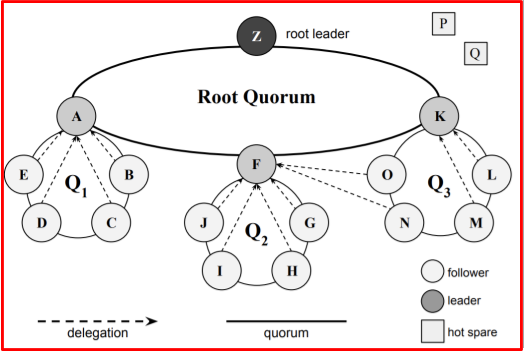
\includegraphics[width=8cm]{figure_3_root_quorum.png}
\label{fig:root_quorum}
\end{figure}

The root quorum's primary responsibilities are mapping replicas to individual 
subquorums and mapping subquorums to tags within the namespace.
Each such map defines a distinct epoch, $e_x$, a monotonically increasing 
representation of the term of the configuration of subquorums and tags, 
$Q_x$.
The root quorum is a consensus group consisting of subquorum leaders.
Somewhat like subquorums, the membership of the root quorum is not defined 
by the quorum itself, but in this case by leader election or peer delegations 
in the lower tier.
While the root quorum is composed of all replicas in the system, only this 
subset of replicas actively participates in root quorum decision making,
in the common case.

The root quorum partitions (shards) the namespace across multiple 
subquorums, each with a disjoint portion as its scope.
The namespace is decomposed into a set of tags, $T$ where each tag $t_i$ 
is a disjoint subset of the namespace.
% Ben: above Pete says T=t_i summation

Tags are mapped to subquorums in each epoch, $Q_x \mapsto T_x$ such that 
$\forall t \in T_x$ $\exists! q_{i,x} \mapsto t$.
The intent of subquorum localization is ensure that the \emph{domain} of 
a client, the portion of the namespace it accesses, is entirely within 
the scope of a local, or nearby, subquorum.
To the extent that this is true across the entire system, each client 
interacts with only one subquorum, and subquorums do not interact at all 
during execution of a single epoch.
This \emph{siloing} of client accesses simplifies implementation of 
strong consistency guarantees and allows better performance at the cost 
of restricting multi-object transactions.
We use agility to attempt to get this, but allow multi-object transactions.

\subsection{Delegated Voting}
% This is about root quorum operations 
From a logical perspective, the root quorum's membership is the set of 
all system replicas, at all times.
However, running consensus elections across large systems is inefficient 
in the best of cases, and prohibitively slow in a geo-replicated 
environment.
Root quorum decision-making is kept tractable by having replicas 
\emph{delegate} their votes, usually to their local leaders, for a finite 
duration of epochs.
With leader delegation, the root membership effectively consists of the 
set of subquorum leaders.
Each leader votes with a count describing its own and peer votes from its
subquorum and from hot spares that have delegated to it.
A quorum leader is elected to indefinitely assign log entries to slots 
(access operations for subquorums, epoch configurations for the root 
quorum).
If the leader fails, then so long as the quorum has enough online peers, 
they can elect a new leader.
When a failed leader comes back online, it rejoins the quorum as a 
follower.
The larger the size of the quorum, the more failures it is able to 
tolerate.

Delegation ensures that root quorum membership is always the entire 
system and remains unchanged over subquorum leader elections and even 
reconfiguration.
Delegation is essentially a way to optimistically shortcut contacting 
every replica for each decision.
Subquorum repartitioning merely implies that a given replica's vote 
might need to be delegated to a different leader.
To ensure that delegation happens correctly and without requiring 
coordination, we simply allow a replica to directly designate another 
replica as its delegate until some future epoch is reached.
Replicas may only delegate their vote once per epoch and replicas are 
not required to delegate their vote.
To simplify this process, during configuration of subquorums by the 
root quorum, the root leader provides delegate hints, e.g. those 
replicas that have been stable members of the root quorum without 
partitions.
When replicas receive their configuration they can use these hints 
to delegate their vote to the closest nearby delegate if not already 
delegated for the epoch.
If no hints are provided, then replica followers generally delegate 
their vote to the term 1 leader and hot spares to the closest subquorum 
leader.

Delegation does add one complication: the root quorum leader must 
know all vote delegations to request votes when committing epoch 
changes.
We deal with this issue by simplifying our protocol.
Instead of sending vote requests just to subquorum leaders, 
\textbf{the root quorum leader sends vote requests to all system 
replicas.}
This is true even for \emph{hot spares}, which are not currently 
in any subquorum.
Delegates reply with the unique ids of the replicas they represent 
so that root consensus decisions are still made using a majority of 
all system replicas.

This is correct because vote requests now reach all replicas, and 
because replicas whose votes have been delegated merely ignore the 
request.
We argue that it is also efficient, as a commit's efficiency depends 
only on receipt of a majority of the votes.
Large consensus groups are generally slow, not just because of 
communication latency, but because large groups in a heterogeneous 
setting are more likely to include replicas on very slow hosts or 
networks.
In the usual case for our protocol, the root leader still only needs 
to wait for votes from the subquorum leaders.
Leaders are generally those that respond more quickly to timeouts, so 
the speed of root quorum operations is unchanged.

% what happens if there is only one delegate?

\subsection{Epoch Transitions}
% This is about root quorum operations 

Every epoch represents a new configuration of the system as designated 
by the root leader.
Efficient reconfiguration ensures that the system is both dynamic, 
responding both to failures and changing usage patterns, and minimizes 
coordination by colocating related objects.
An epoch change is initiated by the root leader in response to one of 
several events, including:

\renewcommand{\baselinestretch}{1}
\begin{itemize}
    \item a namespace repartition request from a subquorum leader
    \item notification of join requests by new replicas
    \item notification of failed replicas
    \item changing network conditions that suggest re-assignment of replicas
    \item manual reconfigurations, e.g. to localize data
\end{itemize}
\renewcommand{\baselinestretch}{2}

The root leader transitions to a new epoch through the normal commit 
phase in the root quorum.
The command proposed by the leader is an enumeration of the new subquorum 
partition, namespace partition, and assignment of namespace portions to 
specific subquorums.
The announcement may also include initial leaders for each subquorum, 
with the usual rules for leader election applying otherwise, or if the 
assigned leader is unresponsive.
Upon commit, the operation serves as an \emph{announcement} to subquorum 
leaders.
Subquorum leaders repeat the announcement locally, disseminating full 
knowledge of the new system configuration, and eventually transition to 
the new epoch by committing an \texttt{epoch-change} operation locally.

The epoch change is lightweight for subquorums that are not directly 
affected by the overarching reconfiguration.
If a subquorum is being changed or dissolved, however, the 
\emph{epoch-change} commitment becomes a tombstone written to the logs 
of all local replicas.
No further operations will be committed by that version of the subgroup, 
and the local shared log is archived and then truncated.
Truncation is necessary to guarantee a consistent view of the log within 
a subquorum, as peers may have been part of different subquorums, and 
thus have different logs, during the last epoch.
Replicas then begin participating in their new subquorum instantiation.
In the common case where a subquorum's membership remains unchanged 
across the transition, an \texttt{epoch-change} may still require 
additional mechanism because of changes in namespace responsibility.

\subsection{Elastic Quorum Membership}
% This is about adding or removing nodes from the quorum.
In principle, adding or removing a node from the system simply involves a 
root quorum decision that changes the epoch and reconfigures the system. 
However, unlike other configuration changes, elastic membership has 
implications for safety and fault tolerance, which we will discuss in this 
section.

% what happens if delegates make a change then die before anyone is notified?

\section{Epoch Operations}
% This is about subquorum operations 

\subsection{Remote Accesses}

\subsection{Transactions}

% I don't think we can get away with not talking about this.
% need to coordinate multiple subquorum
% elect a temp leader across all SQs, perform a transaction?
% or appoint a default leader?
% if a transaction is entirely b/n a SQ, piggyback
% acquire locks? or be optimistic?
% starting txn readset, stopping txn, use log changeset to decide
% time element
% won't have TPCC (not something we want to add right now)
% for one SQ case, simple 
% for multiSQ case, partition to SQs? main one waits for decisions of others
% has to be 2PC - notify all SQs that the transaction happened
% leave responsibility to the client?


% 2PC commit:
% BEGIN: specify read and write set to know which sqs are involved. 
% sqs respond with read objects 
% END: write set is sent back to sqs which checks for conflicts
% if no conflicts, COMMIT, otherwise ROLLBACK
% 2PC: Iff multiple sqs involved, need to do the 2PC to confirm 
% transaction is committed. 

% TXs sucks over wide area 
% it's free for one subquourm 
% gets worse for multiple subquourms
% HOWEVER reconfiguration will make TXs better (other systems can't do it bc txn mgr and namespace mgr are orthogonal - can't use info from one axis and use in other axis)

\section{Safety}

% What if stuff goes wrong, how to handle? is this safe? 
% Will we get to an inconsistent state? no
% Will it become unavailable? yes but it takes a disaster

\subsection{Expected Failure}
% Failure is expected.
% Two types of failure: node failure and network failure
% If a machine dies, you can replace it and get back to work.
% Does it interrupt operations? No
% Root quorum is monitoring health to ensure failure doesn't derail the system
% what happens in the face of partitions
% Generally people talk about wide area failure in such a way as to collapse two different types of failure; failures of connection between two regions, and the total isolation of a single region.
% However, treating these two types of failure as distinct opens the possibility of addressing them more flexibly with solutions more appropriate to each case.
% new failure mode - loss of an AZ, this would be bad for HC but ok w/ ePaxos

\subsection{Assassination}
% Worst case is all delegates are destroyed. 
% Are we only as fault tolerant as the number of delegates we have?

\subsection{Nuclear Option}
% Reset and start from beginning; what that looks like and how it occurs.

\section{Consistency and Adaptability}
% What we get out of this

\subsection{Exporting a Global Log}
% We get linearizability because we can externalize a global log ordering of events.

\subsection{Adapting Consistency}
% We can optimize behavior.
% We can have ePaxos manage some objects, have Raft manage others, transition objects as necessary.
% Epoch changes are about adaptability, not just failure recovery; the point isn't to avoid transitions
% Epoch transitions are rare with respect to accesses; if you have a million accesses per second, epoch transitions happen once every two minutes (or once per hour).
% We can strategically cause transitions (give list of heuristics)
% Epoch changes don't have to change the entire system, they can change small parts of the system.
% "Introspection" - look at access patterns and automatically optimize (integrate Vertical Paxos health monitoring with epoch transitions). 

\section{Performance Evaluation}

\subsection{Experimental Setup}

% mention availability zones & placement groups

As shown in figures \ref{fig:raft-epaxos-baseline-1} and
\ref{fig:raft-epaxos-baseline-2}, our implementations of ePaxos and 
Raft are correct.
% Ben: Pete says maybe one or the other

\begin{figure}
\caption{Latency of Raft and ePaxos with 3, 5, and 7 replica quorums}
\centering
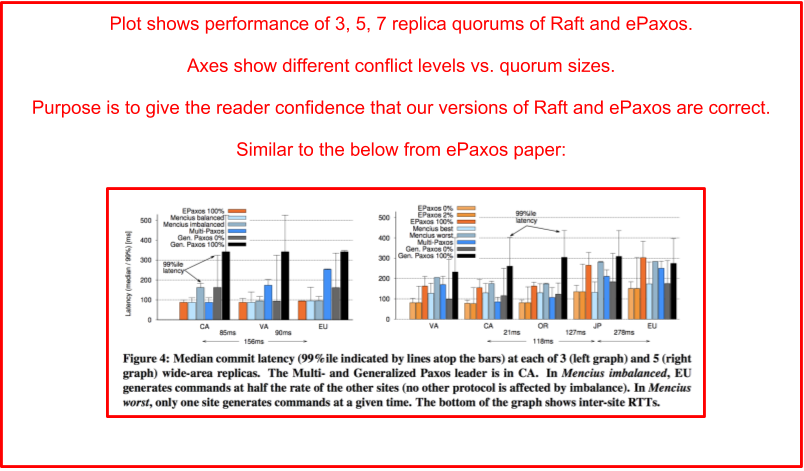
\includegraphics[width=8cm]{raft-epaxos-baseline-1-placeholder.png}
\label{fig:raft-epaxos-baseline-1}
\end{figure}

\begin{figure}
\caption{Throughput of Raft and ePaxos with 3, 5, and 7 replica quorums}
\centering
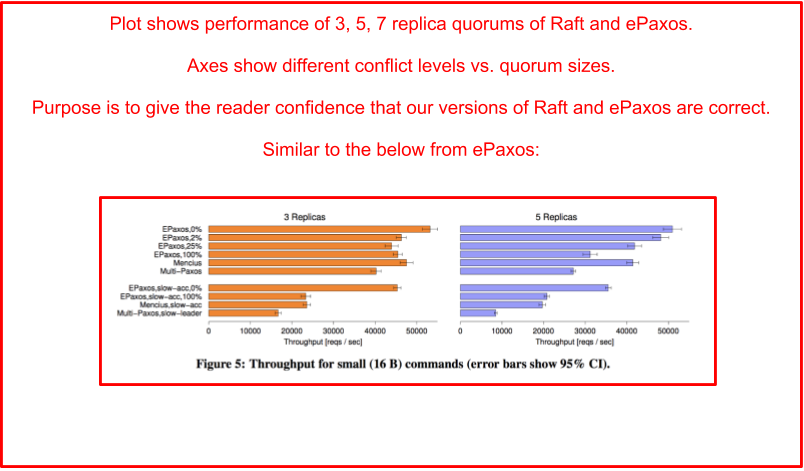
\includegraphics[width=8cm]{raft-epaxos-baseline-2-placeholder.png}
\label{fig:raft-epaxos-baseline-2}
\end{figure}


\subsection{Wide-Area Throughput}

As we see in figure \ref{fig:alia-linear-scaling}, as nodes are added to the system, we get true horizontal scaling. 

\begin{figure}
\caption{Linear scaling of throughput with Alia}
\centering
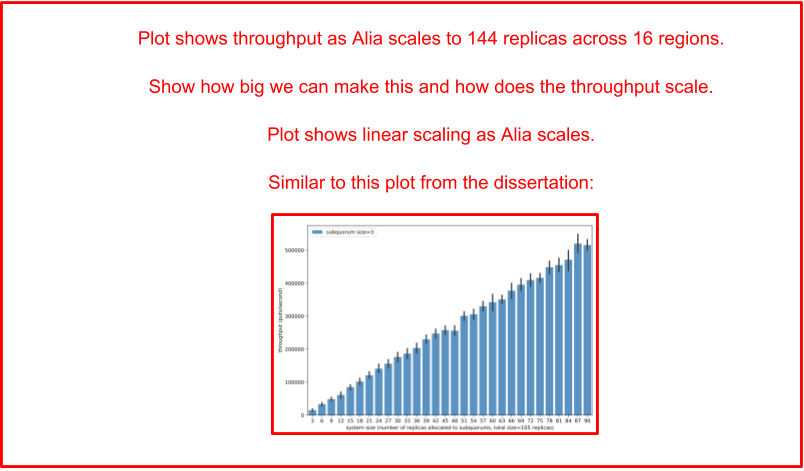
\includegraphics[width=8cm]{16-region-alia-placeholder.png}
\label{fig:alia-linear-scaling}
\end{figure}

\subsection{Commit Latency and Conflicts}

As shown in figure \ref{fig:alia-vs-epaxos}, Alia is has comparable performance
to ePaxos in a zero-conflict context.

\begin{figure}
\caption{Latency of Alia with respect to ePaxos}
\centering
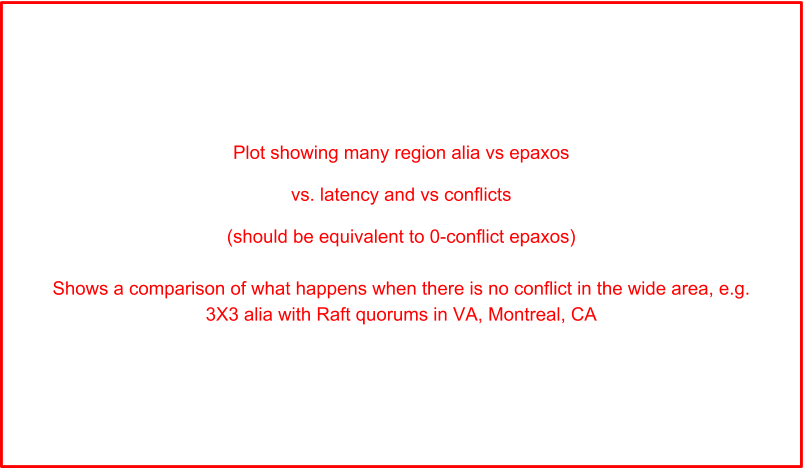
\includegraphics[width=8cm]{alia-vs-epaxos-placeholder.png}
\label{fig:alia-vs-epaxos}
\end{figure}

% We have several types of objects:
% 1. Objects that are only accessed in one AZ 
% 2. Objects that are accessed across AZ but same region (??) 
% 3. Objects accessed on same continent (domestic, e.g. virginia, ohio, montreal)
% 4. Objects accessed across ocean (trans-oceanic, e.g. virginia, london, paris, ohio)
% 5. Truly global objects (e.g. every region or accessed over long haul, e.g. Tokyo, Virginia, London)

Show flexibility by showing variable commit latency depending on type of object, e.g. 
objects are only accessed with a latency subject to the replication links they are 
associated with and no more. 

% No conflict with Raft
% Conflict in ePaxos was access from different regions. We didn't really experience that
% with Raft because it's first come first served. However, if we can do more flexible
% configurations, then these access patterns become even more important and this graph
% shows that we minimize latency to the baseline performance of whatever subquorum is 
% operating. 

\subsection{Fault Tolerance and Adaptability}
% how root quorum decisions influence the system over time

% 0. No need to show what happens when leaders/individual nodes fail 
1. Show what happens when subquorums fail (epoch change recovery),
shown in figure \ref{fig:fault-tolerance}.

\begin{figure}
\caption{Alia is fault tolerant in the face of subquorum failure}
\centering
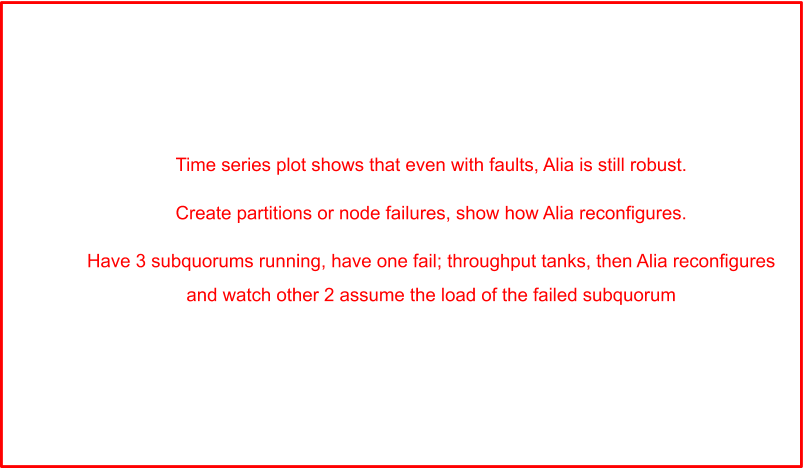
\includegraphics[width=8cm]{fault-tolerence-placeholder.png}
\label{fig:fault-tolerance}
\end{figure}

2. Show sawtooth in figure \ref{fig:sawtooth}: as accesses move to different regions 
% Ben: Pete says we need to make sure we've talked about migrating client access patterns earlier in the paper 
\begin{figure}
\caption{Alia repairs client accesses as they migrate to different regions}
\centering
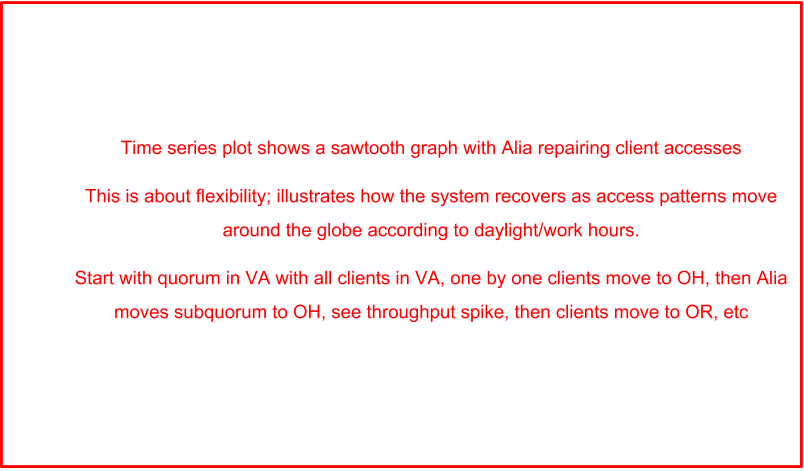
\includegraphics[width=8cm]{sawtooth-placeholder.png}
\label{fig:sawtooth}
\end{figure}

% not exactly sure how to do this, throughput may not be affected?
3. Stretch: show assassination recovery? 

\subsection{Anti-Entropy Optimization}

% this section is all about normal hand-offs. 
% anti-entropy is one optimization, fuzzy epochs is another - do we want to also show 
% the effect of fuzzy epochs in this section?

As we can see in figure \ref{fig:anti-entropy}, anti-entropy improves 
hand-offs and durability.

\begin{figure}
\caption{Anti-entropy improves hand-offs and durability}
\centering
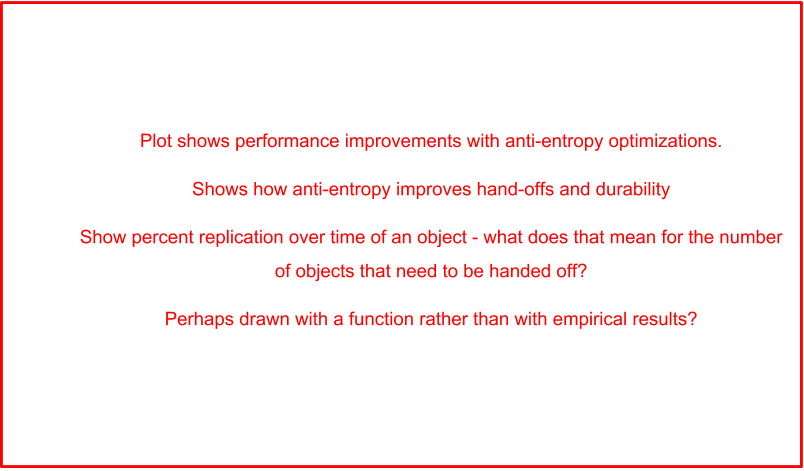
\includegraphics[width=8cm]{anti-entropy-placeholder.png}
\label{fig:anti-entropy}
\end{figure}


\section{Related Work}

Figure \ref{fig:venn-diagram} shows the conditions for which Alia is most
optimal.

\begin{figure}
\caption{Best case scenarios for Alia}
\centering
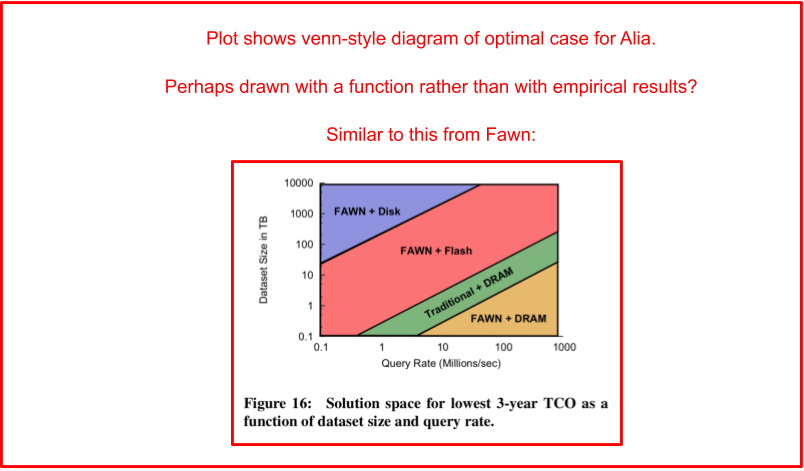
\includegraphics[width=8cm]{venn-diagram-placeholder.png}
\label{fig:venn-diagram}
\end{figure}

% Eris: Coordination-Free Consistent Transactions Using In-Network Concurrency Control

\section{Conclusion}

Where is the data? ITAR and GDPR and other policies are going to become increasingly
influential on the technical landscape.

% \begin{acks}
%     Add acknowledgements as needed.
% \end{acks}

\bibliographystyle{ACM-Reference-Format}
\bibliography{papers}

\end{document}
